\chapter{Аналитический раздел}

\section{Алгоритм шифрования LZW}

LZW --- алгоритм сжатия, основывающийся на поиске схожих символов в файле.

\subsubsection{Алгоритм:}

\textbf{Кодирование}

\begin{enumerate}
	\item Все возможные символы заносятся в словарь. Во входную фразу X
  заносится первый символ сообщения.
	\item Считать очередной символ Y.
  из сообщения.
	\item Если Y --- это символ конца сообщения, то выдать код для X.
	\item Иначе, если фраза XY уже имеется в словаре, то присвоить входной фразе значение XY и перейти к Шагу 2.
	\item Иначе выдать код для входной фразы X, добавить XY в словарь и присвоить входной фразе значение Y. Перейти к Шагу 2.
\end{enumerate}

\textbf{Декодирование}

\begin{enumerate}
  \item Все возможные символы заносятся в словарь. Во входную фразу X
  заносится первый код декодируемого сообщения.
  \item Считать очередной код Y из сообщения.
  \item Если Y --- это конец сообщения, то выдать символ, соответствующий коду X.
  \item Иначе, если фразы под кодом XY нет в словаре, вывести фразу, соответствующую коду X, а фразу с кодом XY занести в словарь.
  \item Иначе присвоить входной фразе код XY и перейти к Шагу 2.
\end{enumerate}

\clearpage

\chapter{Конструкторская часть}

\section{Разработка алгоритма}

На рисунке \ref{fig:algo} представлена схема алгоритма шифрования LZW.

\begin{figure}[h!]
	\centering
	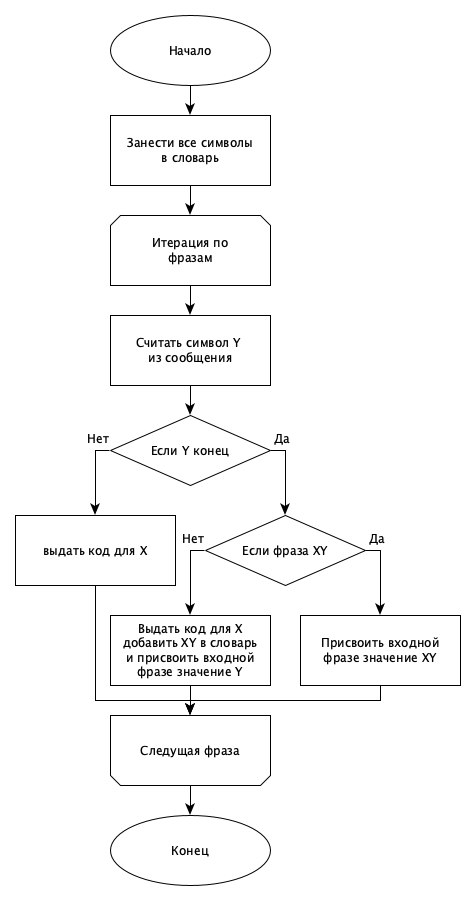
\includegraphics[width=0.6\textwidth]{img/lzf.png}
	\caption{Схемы алгоритма LZW}
	\label{fig:algo}
\end{figure}
